\chapter{Dust Attack}
Il \textit{dust attack} è una tecnica, presente nel mondo delle criptovalute, il cui obiettivo è la 
de-anonimizzazione del proprietario di un $wallet$. L'obiettivo dell'attaccante è di collegare indirizzi diversi tra loro, ovvero riuscire a capire quali indirizzi appartengano ad uno stesso $wallet$.\\

\section{Strategia di attacco}
La strategia usata dagli attaccanti è quella di inviare a diversi indirizzi piccoli importi $dust$.\\
In Bitcoin, il termine $dust$ si riferisce agli importi inferiori alla $fee$ minima richiesta per spenderli in una transazione. Come specificato in \cite{BtcDev}, un
importo è considerato $dust$ se è inferiore alla soglia di 546 satoshi.\\
Per effettuare il \textit{dust attack} quindi è necessario avere a disposizione una certa quantità di bitcoin da poter dividere in centinaia, o migliaia, di output $dust$.
L'attaccante invia questi piccoli importi nella speranza che vengano spesi successivamente in una nuova transazione insieme ad altri indirizzi, poiché è raro che gli indirizzi di input appartengano a più utenti, si presume che tutti gli indirizzi appartengano a una sola persona; quindi sono collegati tra loro.
\begin{figure}[h!]
    \centering
    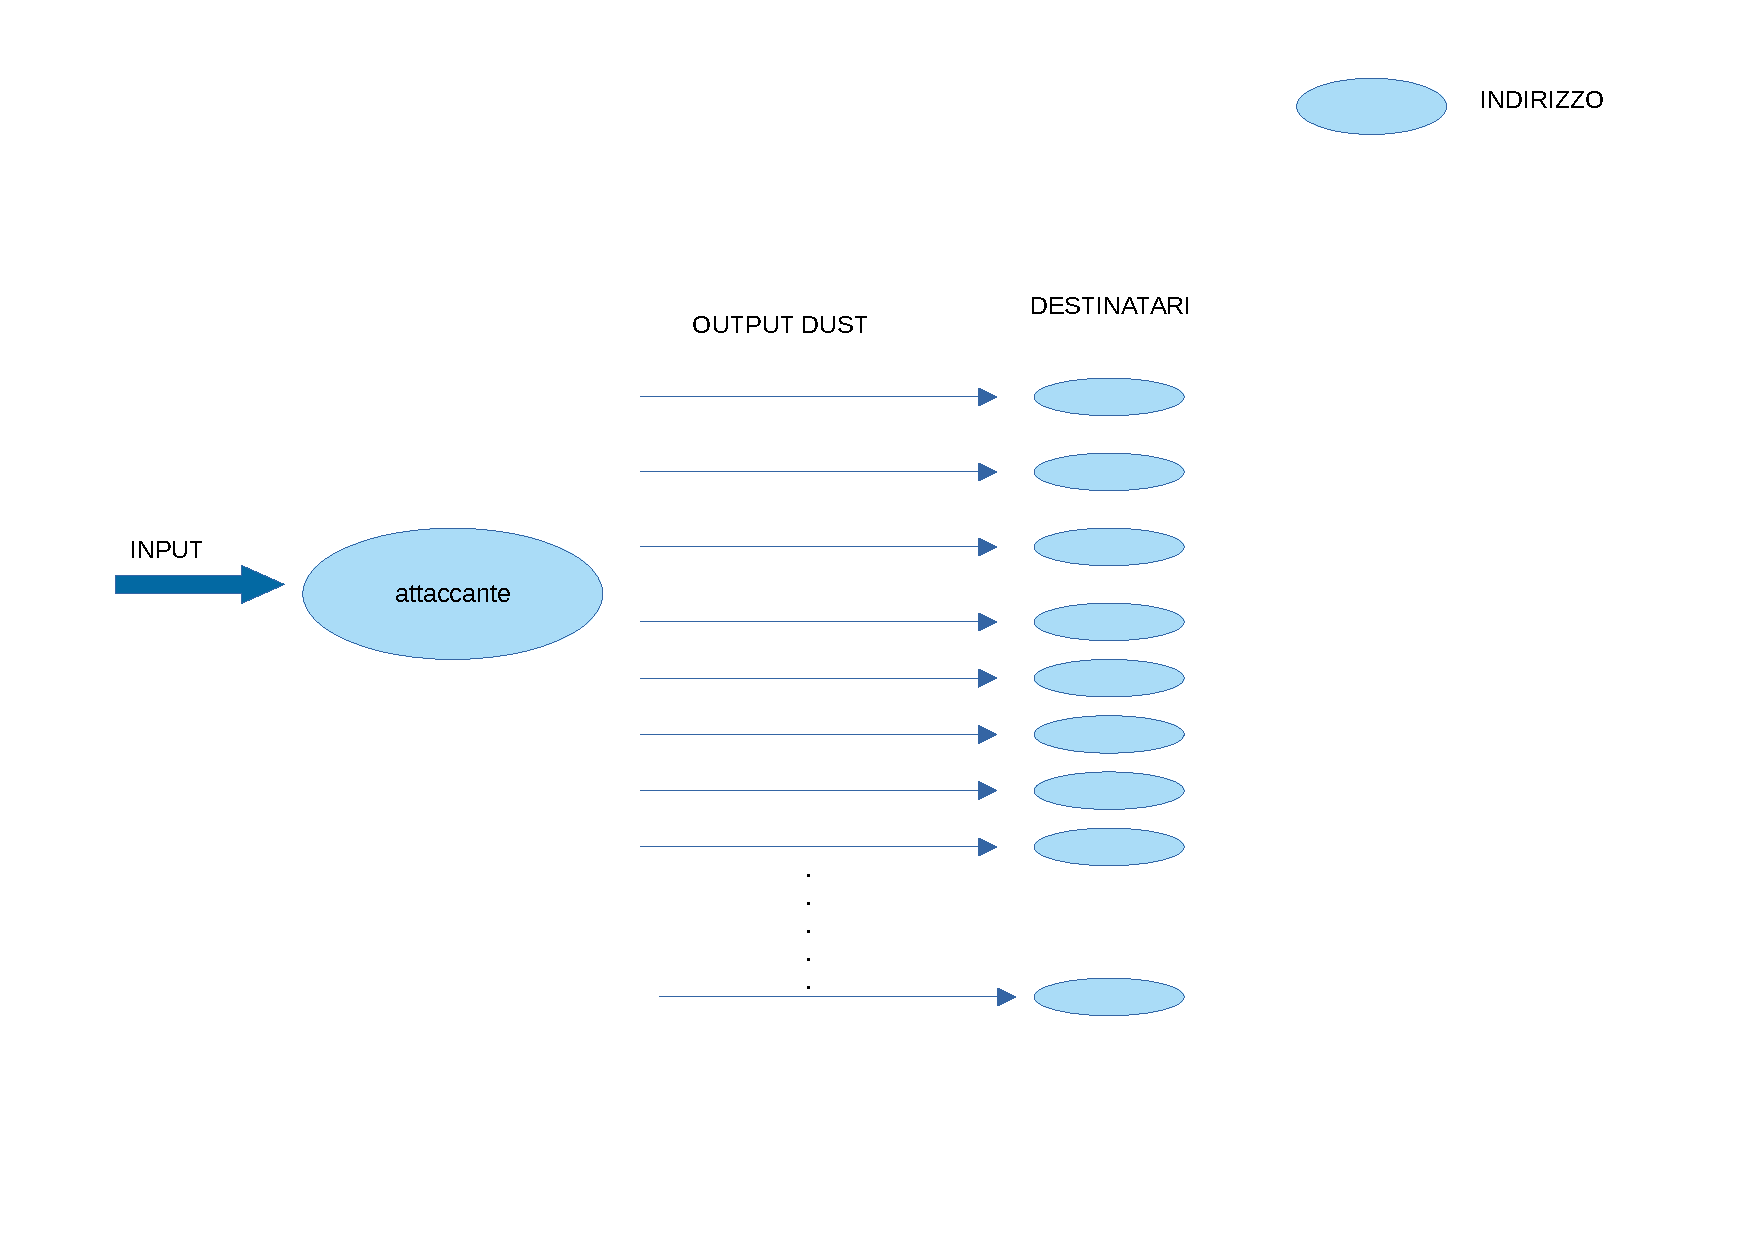
\includegraphics[scale=0.5]{Images/dust_attack.pdf}
    \caption{Schema Dust Attack}
    \label{fig:Dust_attack}
\end{figure}
\FloatBarrier
Una volta effettuato l'attacco possono esserci tre possibili esiti: 
    \begin{enumerate}
        \item attacco di successo;
        \item attacco fallito;
        \item $dust$ bruciato.
    \end{enumerate}
Nel primo caso la vittima genera una transazione in cui spende l'importo $dust$ ricevuto insieme ad almeno un altro dei suoi indirizzi. L'attaccante può quindi collegarli e capire che appartengono alla stessa persona.\\\\
\begin{figure}[h!]
    \centering
    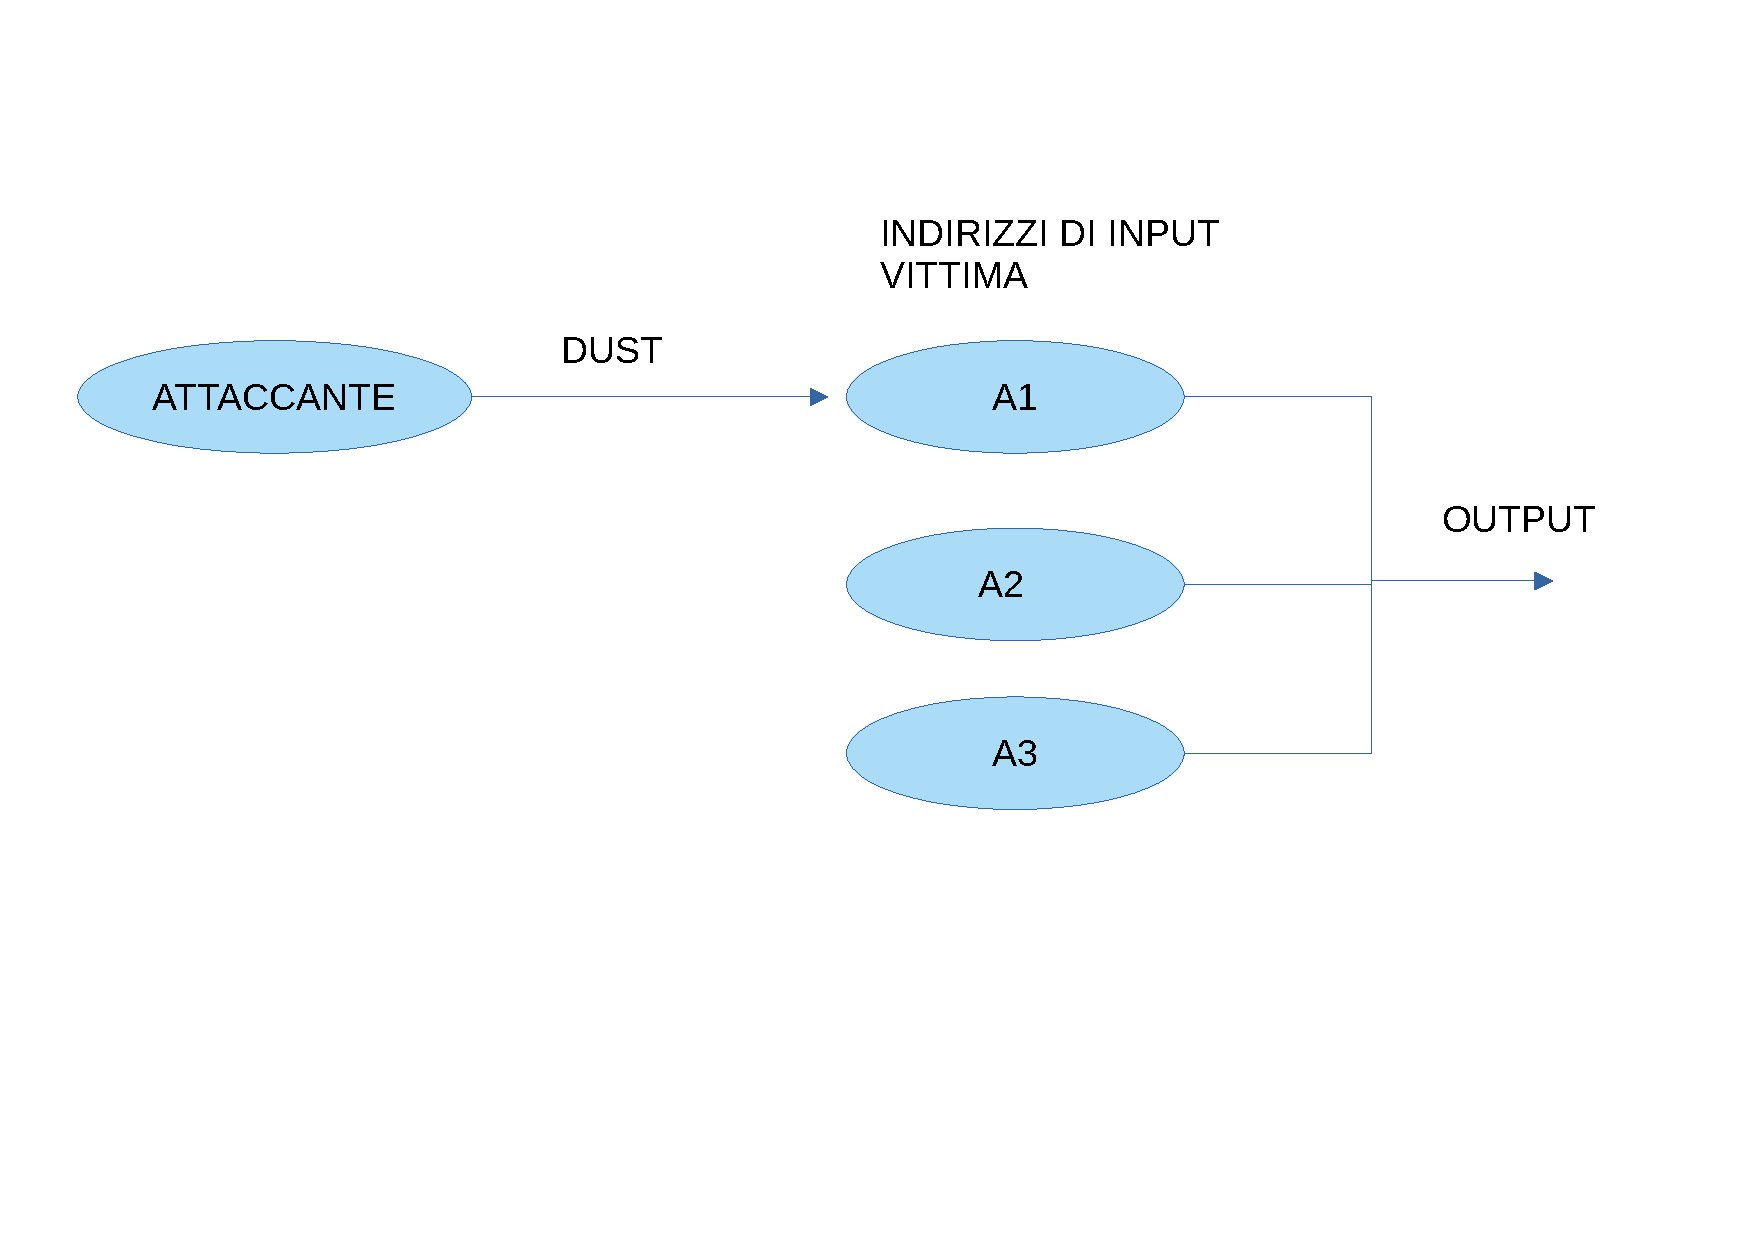
\includegraphics[scale=0.4]{Images/successo.pdf}
    \caption{Schema Attacco di Successo}
    \label{fig:success}
\end{figure}
\FloatBarrier
Nel secondo caso invece l'importo è stato speso in una transazione dove sono presenti più input ma tutti legati allo stesso indirizzo. In questa situazione l'attaccante non collega indirizzi diversi e quindi fallisce nel tentativo di de-anonimizzazione. 
\begin{figure}[h!]
    \centering
    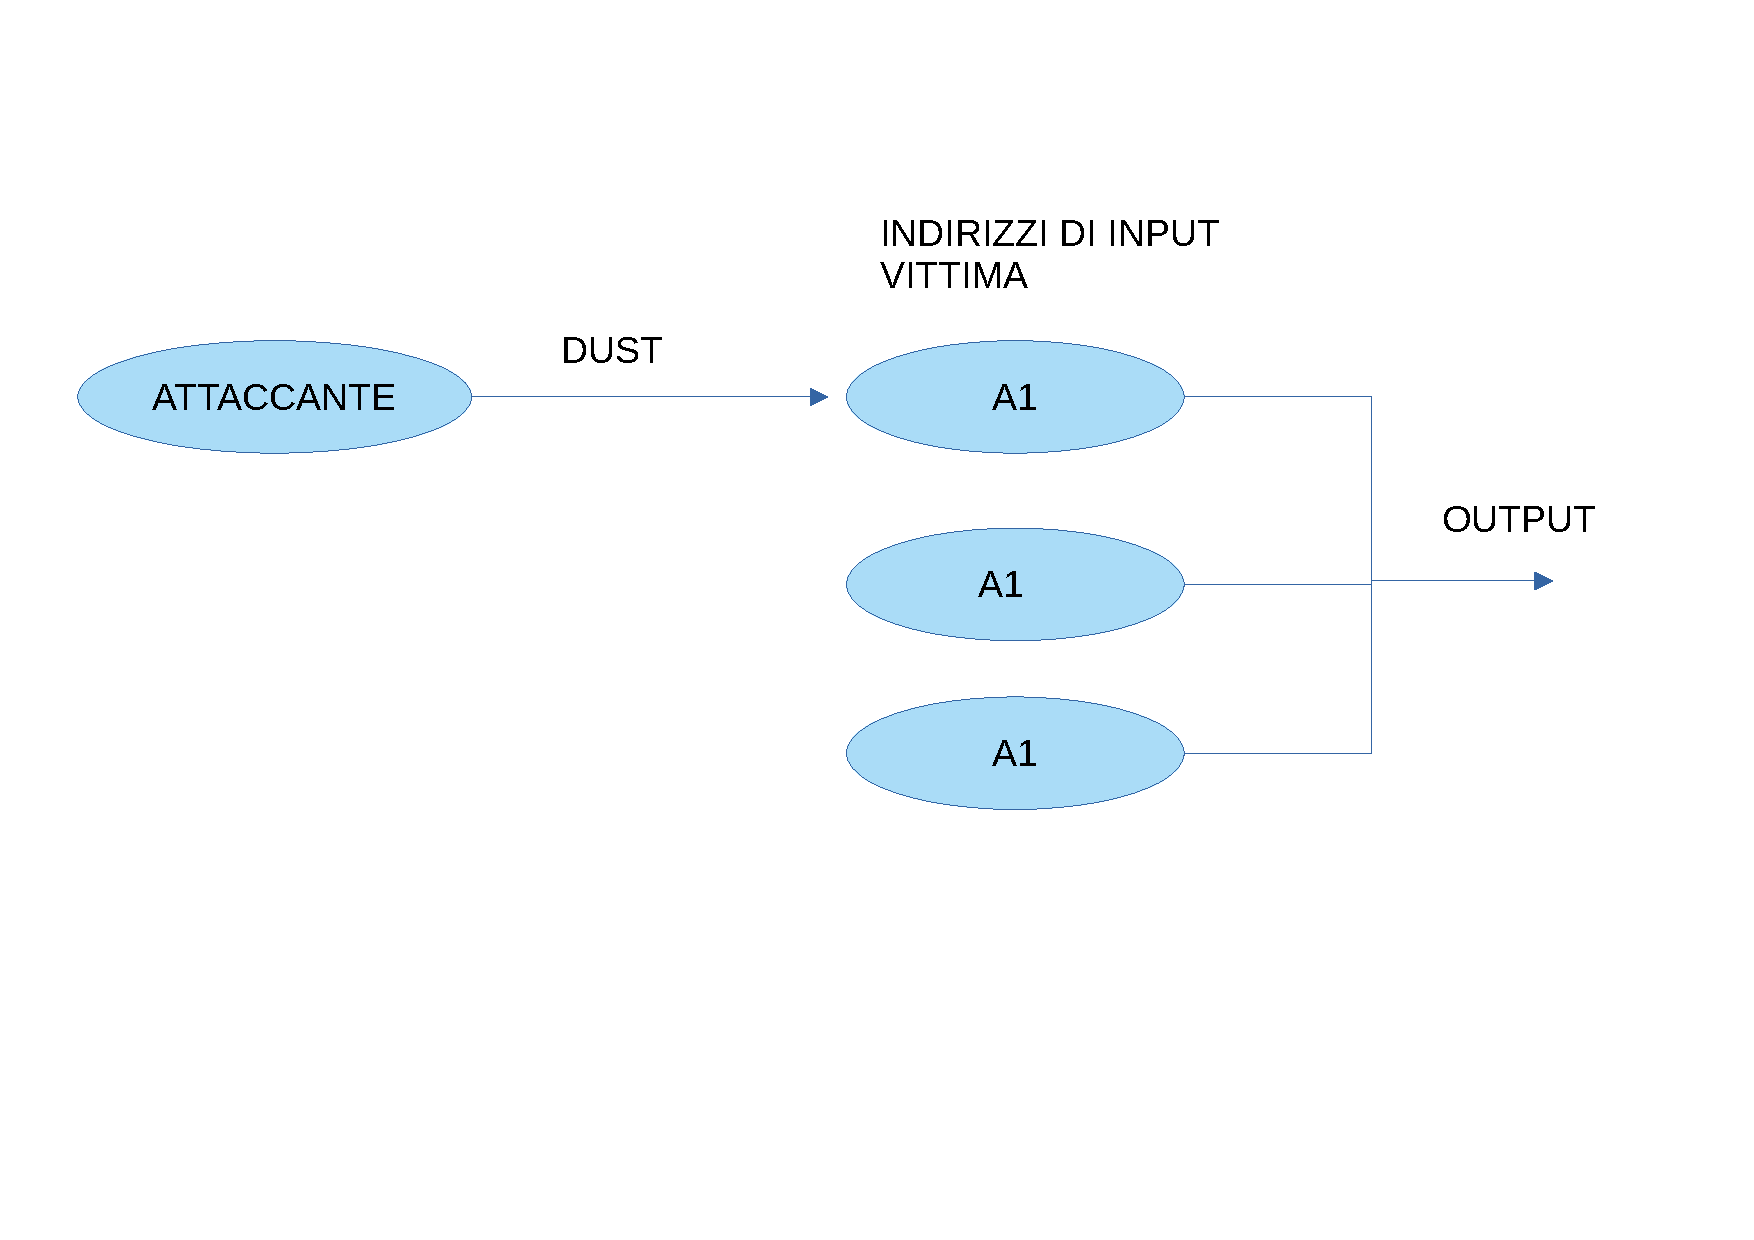
\includegraphics[scale=0.35]{Images/fallimento.pdf}
    \caption{Schema Attacco Fallito}
    \label{fig:Dust_attack}
\end{figure}
\FloatBarrier
Il \textit{dust attack} quindi risulta più efficace soprattutto contro gli indirizzo che hanno un bilancio complessivo pari a zero proprio perchè obbliga la vittima a spendere la cifra ottenuta con altri suoi indirizzi diversi.\\\\
Terzo e ultimo caso semplicemente la vittima non spende il $dust$ ricevuto troncando l'attacco sul nascere.\\\\
Bisogna specficare che il \textit{dust attack} non permette di rubare fondi di altri utenti nè permette di scoprire le informazioni personali, per esempio nome e cognome, della vittima ma permette di ricavare un'importante informazione che può essere usata in seguito per effettuare attacchi più pericolosi.

\section{Conseguenze}
Come detto prima la de-anonimizzazione di per sé non costituisce un problema. Può diventarlo se viene usata come mezzo per altri tipi di attacchi. 
\todo{spiegare conseguenze, tipo exchange e articolo prof di francesco}
\legame indirizzo ip o indirizzo identità tramite exchange
\section{Contromisure}
Due metodi per contrastare il \textit{dust attack} sono:
    \begin{enumerate}
        \item non spendere l'importo $dust$ ricevuto; 
        \item spendere il $dust$ tramite servizi di "dust collecting". 
    \end{enumerate}
La prima soluzione, semplice ed efficace, permette di troncare l'attacco sul nascere. Infatti se il $dust$ non viene speso l'attaccante non potrà mai collegare gli indirizzi. 
Questo metodo può esserre effettuato in diversi software wallet; per esempio Samurai Wallet\cite{SamuraiWallet}, nel 2018, consigliò ai suoi utenti, possibili vittime di \textit{dust attack},  di contrassegnare come "do not spend" le UTXO in questione.\\\\
La seconda soluzione riguarda i servizi di "dust collecting", per esempio Dust-B-Gone\cite{Dbg}.
L'obiettivo di questo meccanismo è di impedire la de-anonimizzazione tramite la generazione di una singola transazione dove gli input $dust$ provengono da utenti diversi. L'importo complessivo viene trasformato in $fee$ per i miners. \\Siccome gli indirizzi di input appartengono a persone differenti, l'attaccante fallisce nel tentativo di de-anonimizzazione.
\textbf{mettere un immagine esempio di dust collecting}